    \section{Versuchsaufbau}
        Um den Versuch durchführen zu können wird eine Schaltung verwendet die man auch im Skript von Herrn Dörr aus Elektronik 1 finden ist (Seite 79). 
         \begin{figure}[h!]
            \centering
            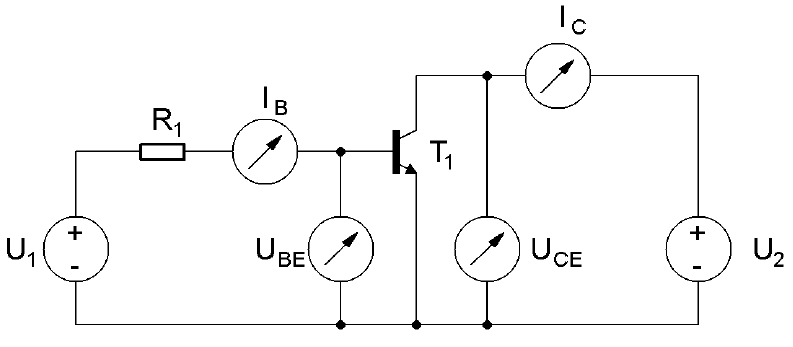
\includegraphics[width=9cm]{Bilder/npn_transistorschaltung.PNG}
            \caption{Schaltung zur Aufnahme der Kennlinien eines NPN-Transistor}
            ~\label{fig:npn_transistor}
         \end{figure}
        